\subsection{Travail sur frochet/quiceh}

\subsubsection{Implémentation de la FFI}

Le code de frochet/quiceh est une bibliothèque, c'est-à-dire que ce code seul ne fait rien, il fournit seulement des fonctionnalités qui peuvent être utilisées dans d'autres programmes.
Un de ces programmes est cURL. cURL est un logiciel permettant d'effectuer des requêtes HTTP en ligne de commande. C'est un logiciel très important pour les développeurs sous Linux, car il est utilisé par des milliers d'autres logiciels.
cURL utilise cloudflare/quiche comme base pour effectuer des requêtes HTTP/3. Or Daniel Stenberg, le développeur principal de cURL se plaint régulièrement des performances d'HTTP/3\up{\cite{stenberg-complaining}}. Cela fait de cURL un choix parfait pour expérimenter le remplacement de cloudflare/quiche par frochet/quiceh et mesurer le gain de performances.

cURL est écrit en langage C tandis que frochet/quiceh est écrit en Rust, il a donc fallu écrire une FFI dans frochet/quiceh pour fournir à cURL une version C des fonctions de Quiceh.
On trouve près de 3500 fonctions dans le code de Quiceh; fort heureusement il n'est pas nécessaire d'écrire une interface C pour chaque fonction de Quiceh. Seules les fonctions utilisées par les programmes externes comme cURL doivent bénéficier d'une FFI, la plupart des fonctions sont des fonctions internes à Quiceh qui n'ont pas besoin d'interface C.
De plus, comme frochet/quiceh est dérivé du code de cloudflare/quiche, la plupart de la FFI était déjà écrite, il fallait écrire la FFI pour toutes les nouvelles fonctions de QUIC VReverso qui fonctionnent sans copie.

\begin{figure}[H]
    \centering
    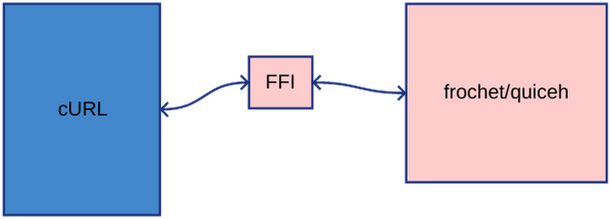
\includegraphics[height=0.15\textheight]{figures/curl_ffi_quiceh.png}
    \caption{La FFI est un morceau de code entre 2 projets écrits dans des langages différents}
\end{figure}

La FFI doit être écrite en langage Rust, n'ayant jamais fait de Rust auparavant, j'ai dû me former sur le langage et la syntaxe de ses FFI. Une fois ceci fait, j'ai pu rapidement écrire la dizaine de fonctions requises par cURL, en les testant non pas sur cURL mais sur un client HTTP très minimaliste en C que j'ai conçu pour l'occasion.

\subsubsection{Portage de frochet/quiceh dans cURL}

Une fois les fonctions de la FFI écrites dans frochet/quiceh, il fallait modifier le code de cURL pour les utiliser.
Malheureusement, cela ne pouvait se résumer à remplacer les fonctions de cloudflare/quiche par celles de frochet/quiceh. Le code de cURL n'était pas du tout conçu pour utiliser les interfaces zéro copie.
cURL copie tous les buffers qu'il reçoit et qu'il doit envoyer dans une queue interne. Si l'on utilise les fonctions de frochet/quiceh dans ce contexte, les données vont se retrouver corrompues car les buffers sont réutilisés.
On peut contourner le problème en copiant systématiquement les buffers dans de nouveaux avant de les ajouter à la queue, mais si l'on fait ça on déplace la copie depuis Quiche vers cURL au lieu de vraiment retirer cette copie.

\begin{figure}[H]
    \centering
    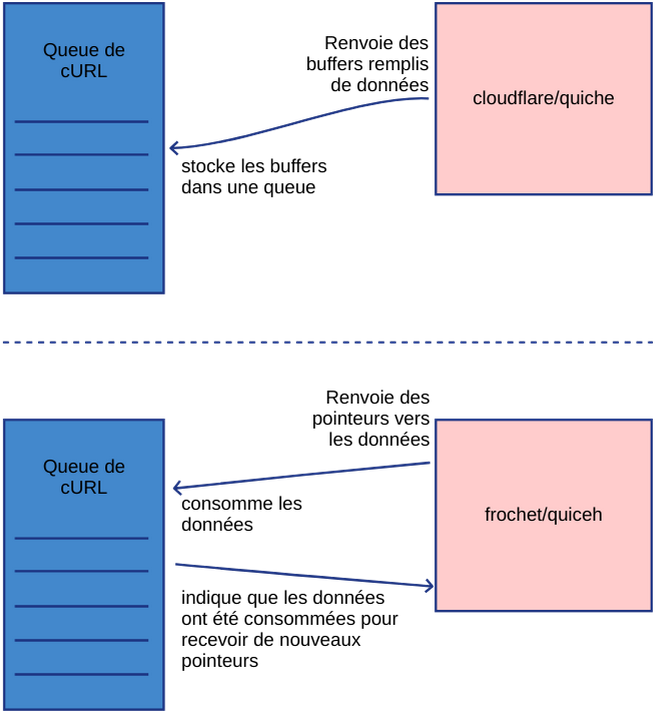
\includegraphics[height=0.37\textheight]{figures/curl_queue.png}
    \caption{\small{La différence de fonctionnement entre cloudflare/quiche et frochet/quiceh rend la queue de cURL inadaptée, car il faudrait copier les données pour les consommer.}}
\end{figure}

Pour mesurer un vrai gain de performance, la seule solution était de trouver un moyen de contourner la queue de cURL lorsqu'on utilise QUIC VReverso. À noter qu'il faut aussi garder l'ancienne queue et l'ancien fonctionnement pour le cas où le pair négocie QUIC V1 plutôt que QUIC VReverso.

En pratique, en mode zéro copie, frochet/quiceh se comporte presque comme la queue de cURL. On peut donc simplement désactiver l'enregistrement dans la queue quand QUIC VReverso a été négocié et changer le moment où la queue est lue pour ne pas récupérer les données depuis la queue, mais depuis frochet/quiceh directement.
Malheureusement, les données à cet endroit sont encore copiées pour être envoyées à une autre partie de cURL. Pour vraiment faire du zéro copie, il aurait fallu supprimer cette copie, mais cela impliquerait de changer presque l'intégralité de l'architecture de cURL, ce qui n'est pas envisageable, nous avons donc décidé d'en rester là et de mesurer les performances à partir de ce point.

\subsubsection{Mesure du gain de performance}

En théorie, mesurer l'écart de performance est facile, il suffit de télécharger un gros fichier, disons 10 Go avec curl + cloudflare/quiche et de chronométrer le temps pris, puis de faire la même chose avec curl + frochet/quiceh, puis faire la différence des deux temps pour connaître le gain. Idéalement il faut faire les mesures plusieurs fois pour faire une moyenne et avoir une mesure plus précise.

Malheureusement, nous pouvons prévoir avant toute mesure que le gain de performances du zéro copie ne sera pas transcendant, on peut s'attendre à voir entre 2 et 3\% d'amélioration sur le temps total. Mais le temps total qu'on mesure lui dépend d'énormément de facteurs et varie de près de 20\% entre chaque lancement.
Si on veut obtenir une mesure précise, du gain en performance, il va falloir trouver une meilleure solution que de chronométrer tout le téléchargement.

\vspace{0.5cm}

Sous Linux, il existe un utilitaire nommé $perf$ qui permet de lancer un programme tout en demandant au kernel de mesurer le nombre de cycles de processeur pris par chaque fonction du programme.
Grâce à cet utilitaire, il est possible de faire des mesures qui d'une part ne sont plus dépendantes de la fréquence du processeur (qui change en permanence) ou de son utilisation par les autres logiciels sur l'ordinateur de mesure, et qui d'autre part permettent d'isoler très précisément le temps passé dans la fonction que l'on cherche à optimiser.

$perf$ n'est pas un outil facile à utiliser, voici pour référence la commande utilisée pour monitorer cURL:

\begin{center}
    \begin{lstlisting}[language=bash]
sudo perf record -e cycles -e sched:sched_switch --switch-events \
    --sample-cpu -m 8M --aio -z --call-graph dwarf ./curl
    \end{lstlisting}
\end{center}

Cette commande génère un fichier $perf.data$ contenant toutes les mesures.
Pour rendre ce fichier lisible par un humain, nous avons choisi d'utiliser le programme $hotspot$\up{\cite{hotspot}} de KDAB.
Ce programme permet d'afficher le résultat de la mesure sous la forme d'un flamegraph, ce qui ressemble à ceci:

\begin{figure}[H]
    \centering
    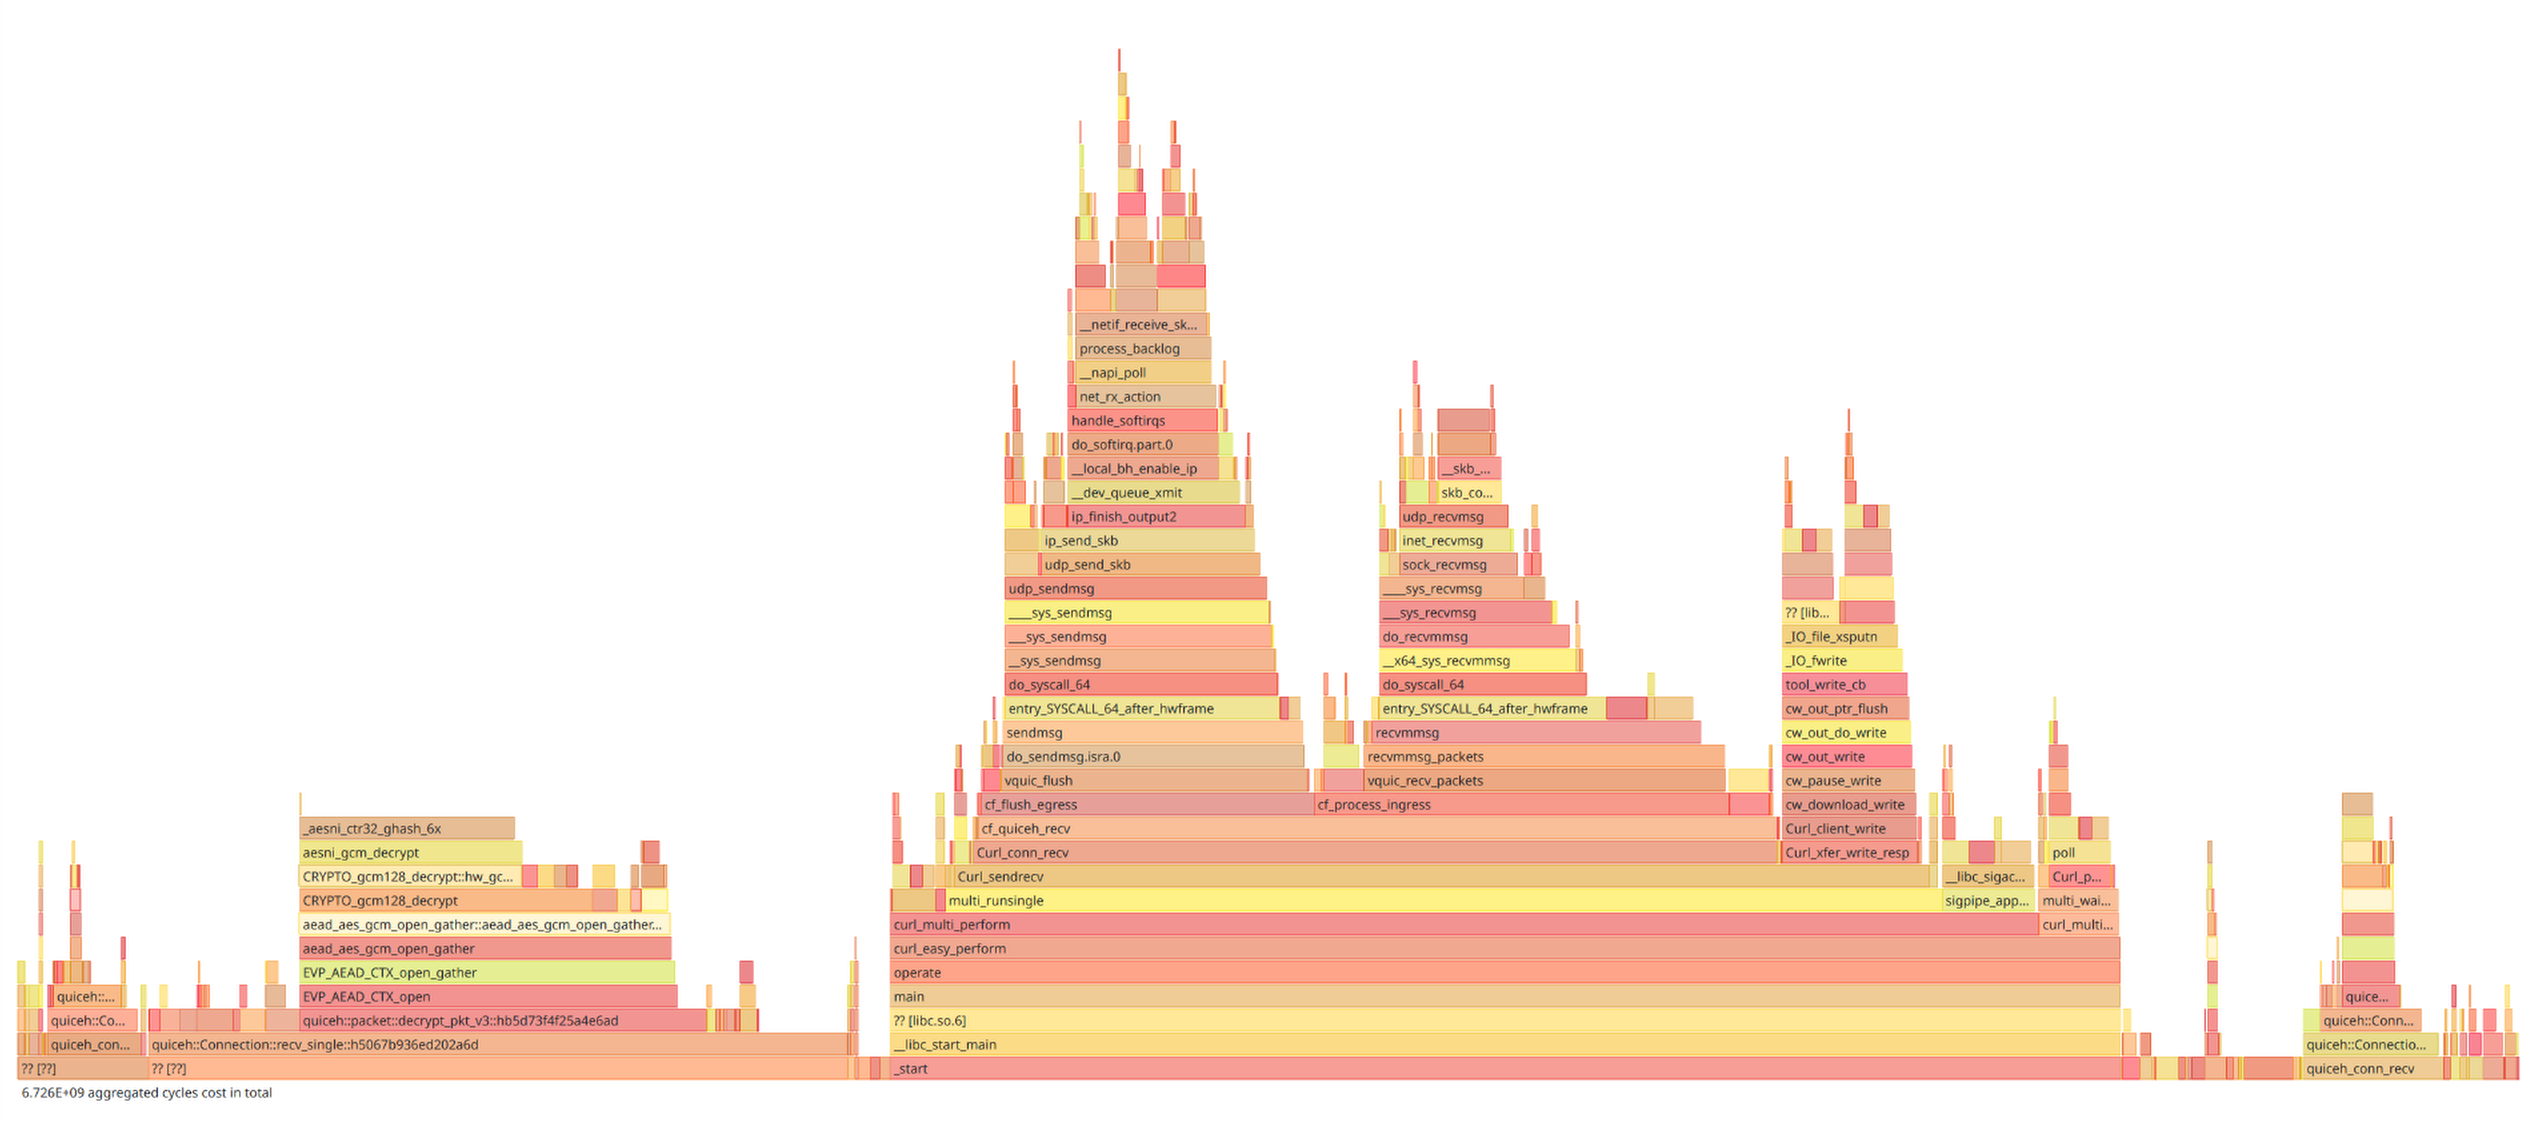
\includegraphics[width=\textwidth]{figures/flamegraph_h3.png}
    \caption{Un flamegraph de curl + frochet/quiceh}
\end{figure}

Ce graphique est une source immense d'information. On y voit avec une grande précision toutes les portions du code de cURL et de quiceh qui consomment une part du temps CPU.
Rapidement on peut voir que 13\% du temps est consacré à la réception de messages (la fonction recvmmsg), 12\% du temps est consacré à l'envoi de messages (la fonction sendmsg) et 32\% du temps est consacré au déchiffrement des messages reçus (la fonction quiceh::Connection::recv\_single). Le reste du temps est réparti dans beaucoup de fonctions, chacune de ces fonctions a un impact presque insignifiant, mais ensembles, ces fonctions représentent tout de même 40\% du temps total. Il faut noter qu'une bonne partie de ce temps n'est pas du tout optimisable, par exemple la cryptographie doit être effectuée à un moment et cela prend beaucoup de temps CPU.

En comparant les flamegraphs de QUIC V1 et QUIC VReverso, on observe bien une copie disparaître, mais le coût de cette copie dans le cas de cURL est marginal. Ce qui est beaucoup plus frappant sur ces graphiques, c'est que malgré le fait que l'on télécharge 1 Go de données et que tout ce qu'on envoie se résume aux accusés de réception, on passe autant de temps à envoyer des messages via sendmsg qu'à recevoir des messages via recvmmsg.

\vspace{0.5cm}

Il n'est vraiment pas normal de passer autant de temps à envoyer des accusés de réception qu'à télécharger du contenu utile, il y a donc potentiellement 10\% du temps CPU de cURL qui pourrait être retiré. 10\% de temps CPU sur un programme utilisé des millions de fois par jours comme cURL, cela représente une quantité d'énergie extrêmement importante. Cette découverte va complètement changer la direction que prenait mon stage, jusqu'à sa fin. Nous avons décidé de rediriger nos efforts à réduire l'impact de l'envoi des accusés de réception dans cloudflare/quiche.

\newpage

\subsection{Implémentation d'accusés de réception différés dans cloudflare/quiche}

\subsubsection{Découverte du problème}

Si cURL passe autant de temps à envoyer des paquets qu'à en recevoir, cela ne peut signifier qu'une seule chose; un accusé de réception est envoyé pour chaque paquet reçu.
Cela peut sembler curieux dans la mesure où Quiche est supposément capable d'envoyer plusieurs accusés de réception en un unique message.

Le fait est qu'en pratique, cette capacité n'est pas vraiment utilisée dans le cas nominal où les paquets arrivent un par un dans l'ordre. En effet, dès qu'un paquet est reçu, un accusé de réception est envoyé, avant d'avoir eu le temps de s'apercevoir qu'un autre paquet reçu entre temps nécessite également un accusé de réception.

\begin{figure}[H]
    \centering
    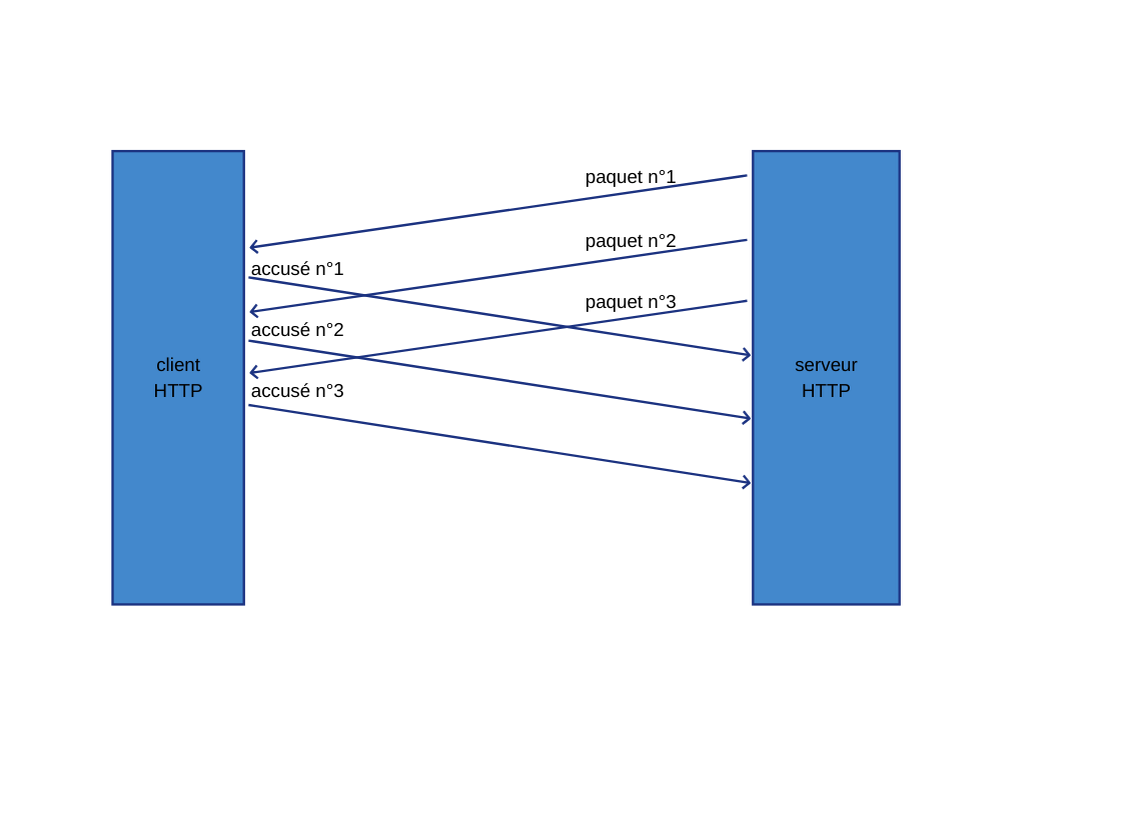
\includegraphics[width=0.8\textwidth]{figures/ack_not_delayed.png}
    \caption{Les accusés de réceptions ne sont pas différés, 6 messages sont générés}
\end{figure}

Cette problématique n'est pas nouvelle, elle a déjà été rencontrée dans le développement de TCP et la solution a été de mettre en place des accusés de réception différés. L'idée étant qu'à la réception d'un paquet, plutôt que d'envoyer immédiatement un accusé de réception, il est plus intéressant d'attendre un cours instant pour voir si l'on reçoit d'autres paquets.

\begin{figure}[H]
    \centering
    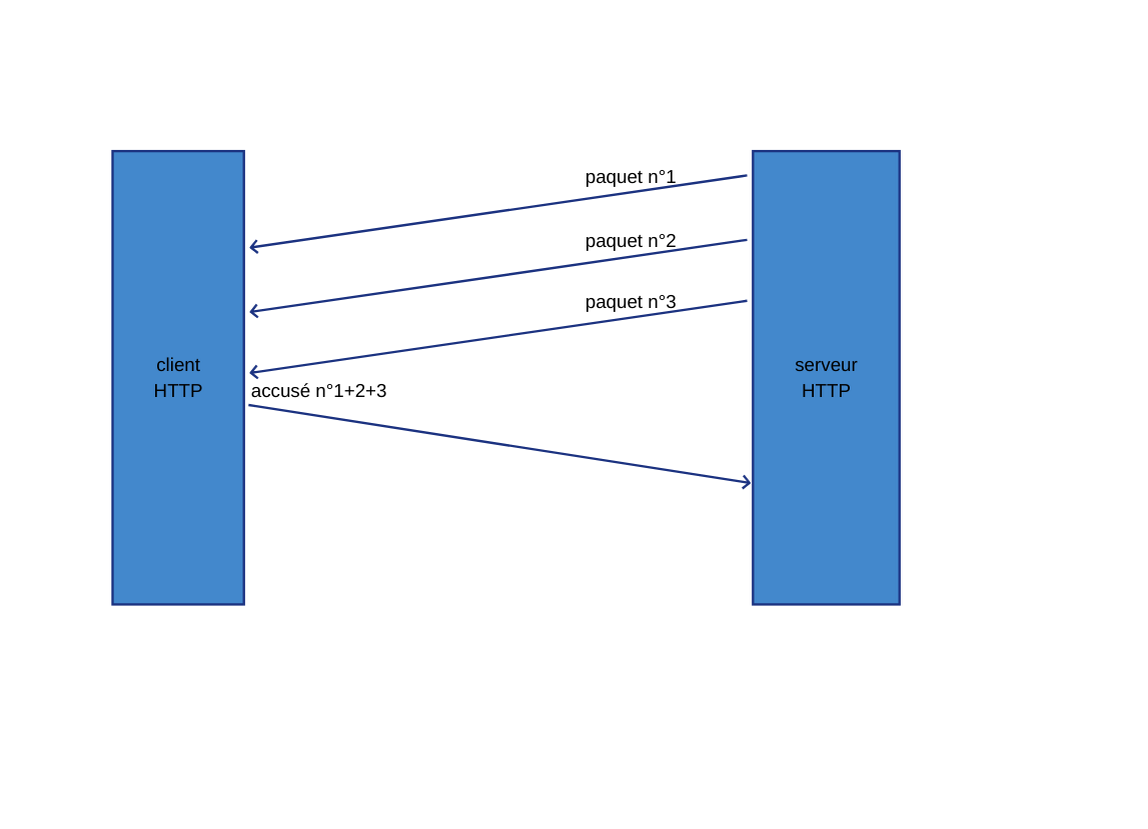
\includegraphics[width=0.8\textwidth]{figures/ack_delayed.png}
    \caption{Les accusés de réceptions sont différés, 4 messages sont générés}
\end{figure}

En introduisant des accusés de réception différés, on réduit le nombre de paquets sur le réseau, ce qui peut permettre d'augmenter le débit. Envoyer moins de paquets c'est aussi chiffrer moins de paquets, car pour rappel, QUIC chiffre les accusés de réception. Or c'est le chiffrement des paquets qui consomme le plus de puissance de calcul.

Bien sûr, cela vient avec un coût. En différant les accusés de réception, l'émetteur met plus de temps à se rendre compte qu'un message a été perdu et mettra plus de temps avant de renvoyer les messages perdus. Tout est donc question de compromis, plus l'on diffère les accusés de réception et plus le protocole est efficace en conditions nominales, mais moins il devient réactif aux pertes de paquets.

\subsubsection{QUIC et les accusés de réception différés}

Le protocole QUIC n'intègre pas à ce jour de mécanismes pour gérer les accusés de réception différés.
Pour implémenter cela, il est nécessaire de pouvoir négocier cette fonctionnalité avec le pair, afin de configurer le délai et les conditions d'attente pour la communication.

Il existe un draft, c'est-à-dire une proposition en attente d'une éventuelle révision pour entrer dans le standard, qui décrit précisément ce mécanisme pour QUIC\up{\cite{draft-ack-frequency}}.
Ce draft est intitulé \guillemotleft QUIC Acknowledgment Frequency \guillemotright. Comme son nom l'indique, son principal changement proposé est l'ajout d'une nouvelle trame de contrôle permettant de négocier la fréquence des accusés de réception en temps réel pour s'adapter au réseau qui peut être changeant.

Après quelques recherches, nous avons découvert qu'il existait un très vieux commit\up{\cite{old-delayed-ack-branch}} de Junho Choi qui avait commencé à implémenter une ancienne version de ce draft.
Le travail sur cet ancien commit n'avait jamais été poursuivi ni intégré à la branche principale de cloudflare/quiche.

Nous avons donc décidé de partir de ce commit comme base, en travaillant directement sur une copie de cloudflare/quiche plutôt que sur frochet/quiceh.

\begin{figure}[H]
    \centering
    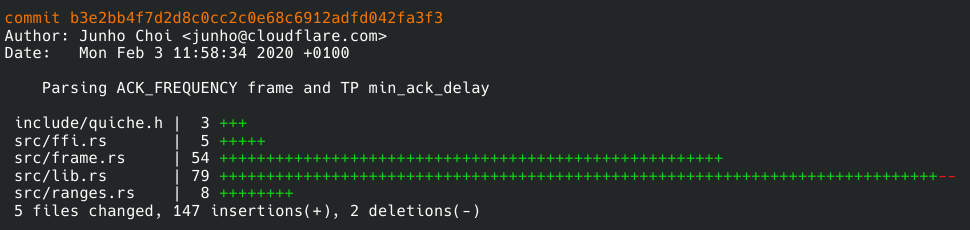
\includegraphics[width=\textwidth]{figures/junho_choi_commit.png}
    \caption{Le commit de Junho Choi, relativement petit, mais très âgé.}
\end{figure}

\subsubsection{Un début difficile avec l'implémentation du draft.}

Le code de cloudflare/quiche ayant énormément changé depuis le commit de Junho Choi, la première étape consistait à porter ce vieux commit vers la version la plus récente de cloudflare/quiche.
Normalement cette opération se fait facilement avec la commande $git~merge$, éventuellement en corrigeant quelques conflits à la main.

Malheureusement, ici, plus de cinq ans s'étaient écoulés depuis le commit et la structure de Quiche avait complètement été modifiée, les changements opérés par le commit ne s'intégraient plus du tout naturellement dans la nouvelle version de Quiche.

Il nous a fallu une journée complète de travail pour porter manuellement toutes les lignes de code du commit de Junho Choi en essayant pour chacune de ces lignes de ne pas introduire de bugs lorsque nous les modifions pour les intégrer dans le nouveau code.

\vspace{0.5cm}

Comme nous pouvions nous y attendre, lors du lancement du code porté, rien ne fonctionnait. Certains problèmes étaient déjà présent dans le commit de Junho Choi. d'autres venaient d'une imcompatibilité au niveau de l'interaction entre l'ancien code et le nouveau, enfin une partie des problèmes n'étaient que des erreurs introduites par le portage manuel, prône aux erreurs.

\vspace{0.5cm}

Quoi qu'il en soit, il aura fallu une semaine pour traquer et réparer tous les problèmes et enfin avoir un code qui se lance et une communication qui s'établie.

\vspace{0.5cm}

Malheureusement, nous n'étions pas au bout de nos peines, car bien que la communication s'établissait, et que les accusés de réception semblaient bien être différés de la durée prévue, le débit était divisé par soixante. Télécharger 1Go prenait maintenant 2 minutes au lieu de 2 secondes.

\subsubsection{Diagnostic du problème de débit.}

Cette perte de performance si impressionnante était vraiment inquiétante. Nous n'avions pas encore implémenté tout le draft, nous n'avions notamment pas de gestion correcte des paquets désordonnés ou perdus, cela pouvait poser des problèmes, mais cela n'expliquait pas du tout une telle baisse des performances, alors que nous effectuions nos essais en local, donc avec aucune perte de paquets en théorie.

\vspace{0.5cm}

Cela pouvait être causé par de nombreuses choses, peut-être que chaque paquet était envoyé 60 fois, peut-être que le serveur refusait d'envoyer un deuxième paquet tant que le premier n'avait pas été acquitté, peut-être que le client ou bien le serveur se mettait en pause à des moments où il y avait des paquets à traiter ou peut-être était-ce autre chose ?

\vspace{0.5cm}

Nous pouvions déjà obtenir quelques informations à l'aide de $perf$ et $hotspot$.

\begin{figure}[H]
    \centering
    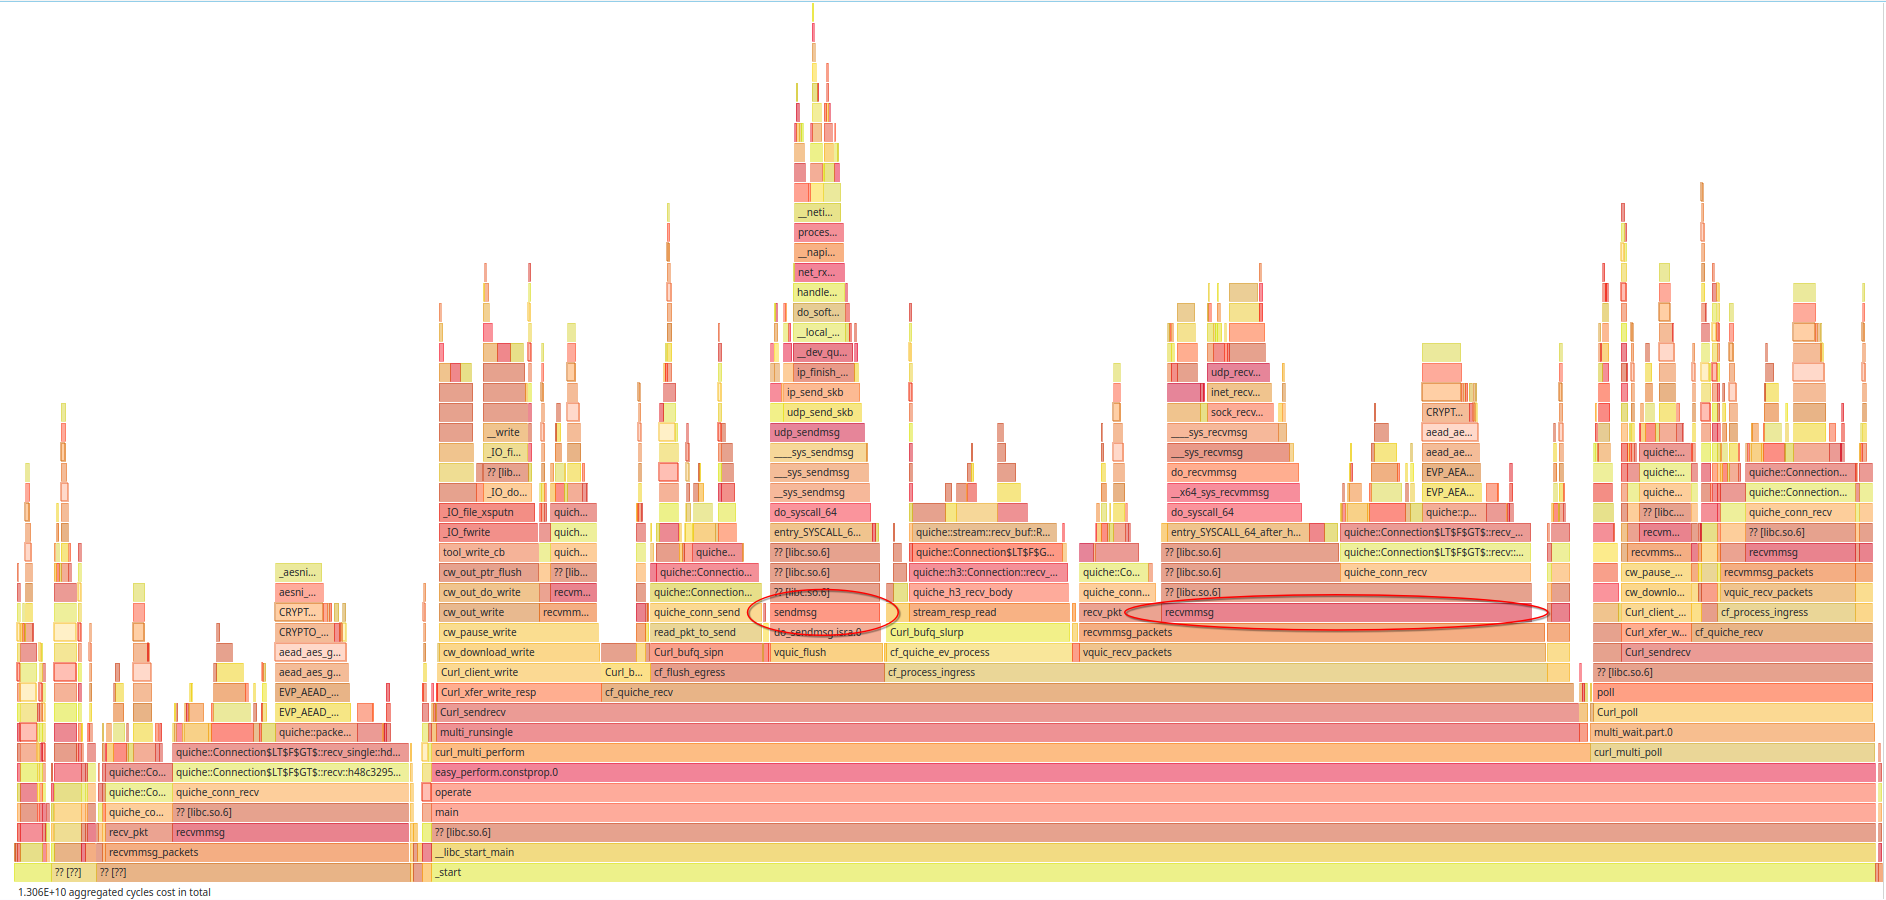
\includegraphics[width=\textwidth]{figures/flamegraph_delayed_ack.png}
    \caption{Flamegraph du téléchargement prenant 2 minutes.}
\end{figure}

Sur ce flamegraph, on voit que les accusés de réception sont bien différés, car les cycles de processeur de sendmsg sont divisés par 5, ce qui est la preuve qu'on envoie 5 fois moins d'accusés de réception.
Cela nous permet d'affirmer que Quiche n'attend pas l'accusé de réception du premier message avant d'envoyer le deuxième.

En cliquant sur les champs, on peut également voir que le nombre de cycles de processeur n'est pas anormalement élevé, ce qui invalide l'hypothèse selon laquelle tous les messages sont envoyés 60 fois.

\vspace{0.5cm}

En mesurant les temps d'inactivité du client et du serveur, nous avons remarqué que l'immense majorité du temps, les deux étaient juste bloqués en attente, sans faire le moindre calcul.

Trouver la source du problème a été une tâche longue et difficile. Ce n'est qu'après avoir relu très minutieusement le draft pour la cinquième fois que nous avons compris que tous nos soucis étaient causé par le contrôle de congestion.

\subsubsection{Le contrôle de congestion, un piège vicieux pour les accusés de réception différés.}

Le contrôle de congestion est une fonctionnalité importante de QUIC, qui est directement héritée de TCP. Le contrôle de congestion sert à améliorer les débits en assurant de ne jamais congestionner le lien.
Pour comprendre ce que fait le contrôle de congestion, il faut comprendre d'où viennent les pertes de paquets sur un réseau IP traditionnel.

Sur internet, tous les équipements sont branchés physiquement les uns aux autres, généralement avec de la fibre optique. Ces liens sont très fiables et il est hautement improbable qu'un paquet soit perdu à cause du lien physique. En revanche, si un routeur est surchargé et ne parviens plus à traiter les paquets suffisamment vite, il va simplement jeter les paquets qu'il n'a pas le temps de gérer.
Presque tous les paquets perdus sur internet viennent de là, des routeurs saturés qui jettent des paquets.

Pour QUIC ou TCP, un paquet jeté génère un gros problème de performance, car il va falloir attendre l'information que le paquet n'est pas arrivé, puis il va falloir le renvoyer. Toute la communication est bloquée lors de cette phase.

Il est donc crucial pour QUIC et TCP de s'assurer de ne pas saturer les routeurs. Pour ce faire, le contrôle de congestion va réduire le débit de l'envoyeur dès qu'il détecte qu'un paquet est perdu.

\vspace{0.5cm}

Le contrôle de congestion de QUIC est un peu plus agressif que celui de TCP et l'une de ses spécificités est qu'il peut réduire le débit avant même qu'un seul paquet soit perdu s'il détecte qu'un accusé de réception a mis un temps plus long que celui attendu à revenir.

Autrement dit, en différant l'envoi des accusés de réception, nous avons indirectement ordonné au contrôle de congestion de QUIC de réduire son débit.
Ceci explique parfaitement le fait que le débit ait été finalement divisé par 60.